\chapter{System Architecture}\label{ch:system_architechture}

The Syllabus is run, logs are generated, Metrics code is run.



Metrics code scrapes the logs, extracts the relevant information and produces a set of numbers which are used to evaluated each Core Capability





\begin{figure}[h]
	\centering
	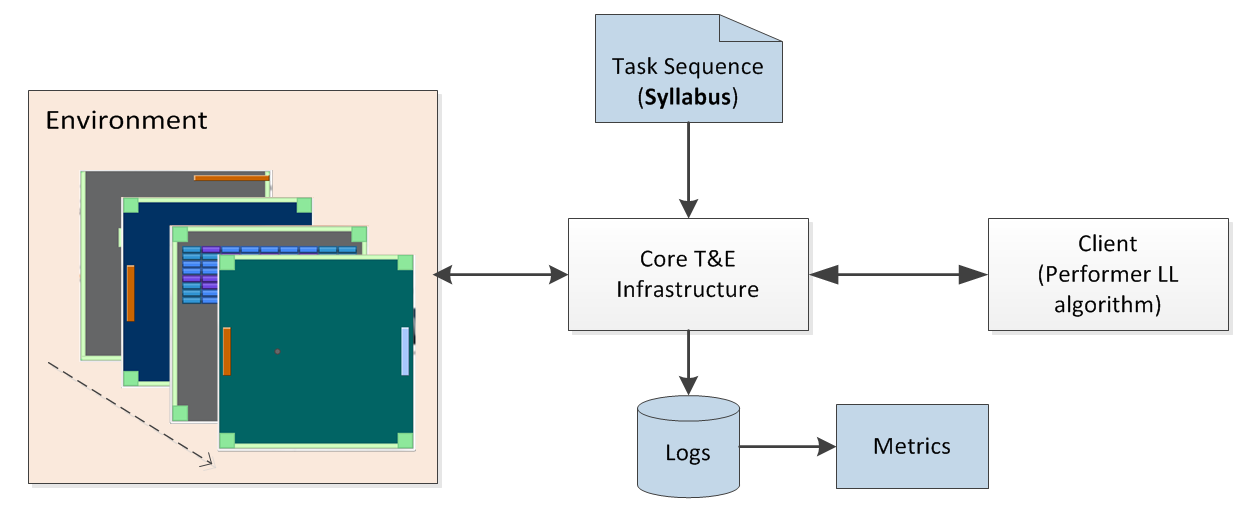
\includegraphics[width=0.85\columnwidth]{sections/figs/metrics_diagram.png}
	\caption{This figure describes the production of Metrics from Log files outputted by the Core Test and Evaluation Framework.}
	\label{fig:system_layout}
\end{figure}



\begin{figure}[h]
	\centering
	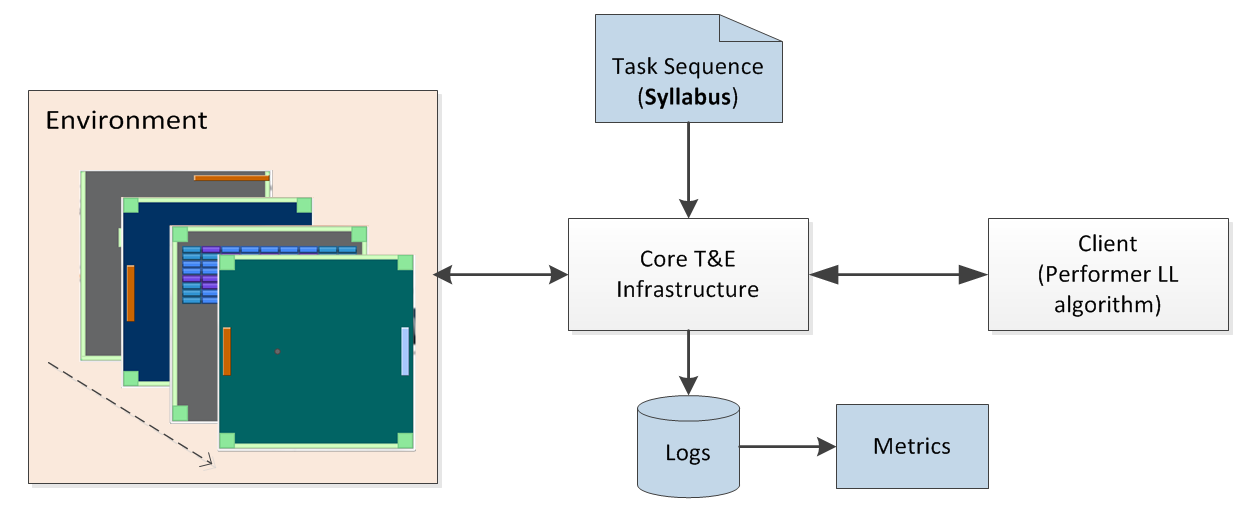
\includegraphics[width=0.85\columnwidth]{sections/figs/metrics_diagram.png}
	\caption{An example log file.}
	\label{fig:system_layout}
\end{figure}
